\label{sec:BDT}
Boosted Decision Trees (BDTs) have a long history in high energy physics and have been used since Ancient Age to identify a variety of signatures [CITATIONS NEEDED]. A decision tree functions by making a seriies of cuts (or decisions) that maximize the separation between signal and background events in a single dimension. Each cut produces a branch in the tree containing independent populations. The depth of three sets the number of decisions a tree will make, and a well-designed tree will have end-nodes that provide relatively pure classification of the inputs. Any series of cuts for identifying events will inevitably mis-classify some events, and there are many strategies for improving the results. A boosted decision tree attempts to improve the classification by creating a new set of data from the improperly classified events and training a new decision tree on these inputs. Each step of re-training with mis-classified events is called a \textit{boost}, and the total prediction for an eventis the weighted sum of predictions from the orignal tree and the boosted trees where each sequential boost recieves a smaller weight in the sum.

The BDT trained for dihiggs detection was built using the xgboost package~\cite{xgboost} and uses events reconstructed using the 'equalDijetMass' reconstruction algorithm. Reconstructed variables include the masses and momentum of the four- and two-body higgs candidates as well as the angular separations between the two Higgs candidates and their consituent jets. Additional event-level variables like the number of selected jets, the number of b-tagged jets, and the missing transverse energy in the event were also considered. All possible varibles were evaluted for individual separation power between signal and background, and the top seventeen variables were used in training. The hyperparameters describing the boosted decision tree were optimized for maximum $S/\sqrt{B}$. The optimal hyperparamters were found to be as follows: multiplicative boost factor of 0.1, maximum tree depth of 9, gamma (minimum loss reduction needed for further partition) of 1.1, and an L2 regularization term of 8.28.

\begin{figure}[!h]
\begin{center}
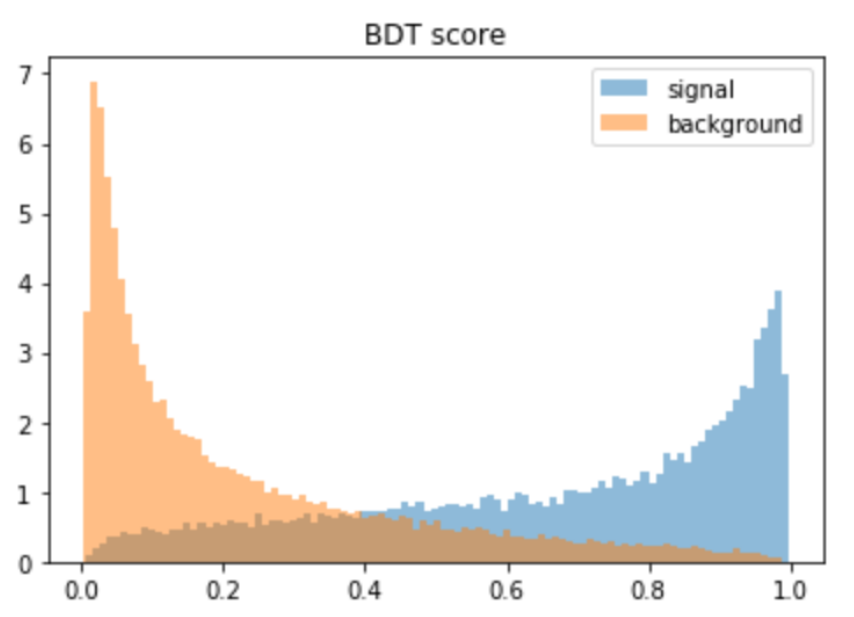
\includegraphics[width=3in]{BDT/bdt_pred}
\caption{Signal predictions of the trained BDT for signal and background samples independent from the training sets.}
\label{fig:bdt_pred}
\end{center}
\end{figure}

The predictions from the optimized BDT are shown in Figure~\ref{fig:bdt_pred}. A maximum significance of 1.84$\pm$0.09 was obtained, yielding 986 signal events and 2.8$\cdot 10^5$ background events. 

\subsubsection{PCA and Clustering Extensions}
Say something about the clustering and how it was dumb and didn't do much. Also the PCA in the BDT and the PCA with clustering.



